
\subsection{Real robot testing and analysis} 

This section details the implementation of the proposed Complete Coverage Path Planning (CCP) algorithm on a real robot platform, addressing both scenarios with and without obstacles. The subsequent analysis of the experimental results is provided. The section is organized into two main parts: Experimental Setup and Results \& Analysis. 

\subsection{Experimental Setup} 

This subsection provides a comprehensive description of the real robot setup, emphasizing the experimental framework within which the tests are conducted.   

\vspace*{6mm}   


The real-world experiments were conducted using a specially designed robot platform equipped with a camera for weed detection upon weed detection by the drone for accuate extractionn, and a GPS module for localization of the robot itself. This robot is specifically engineered to operate in grass fields. The robot can be visualized in (\autoref{fig:real_robot}).   
\begin{figure}[htbp]
    \centering
    % 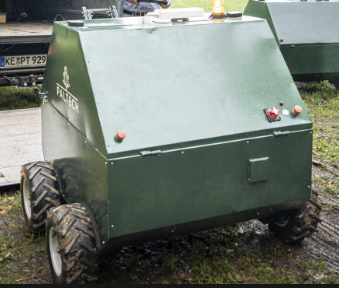
\includegraphics[width=\textwidth]{Images/real_robot/robot.png}
    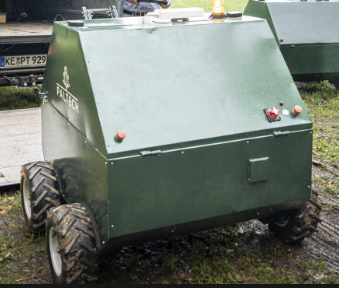
\includegraphics[width=0.5\textwidth]{Images/real_robot/robot.png}
    \caption{Real robot.}
    \label{fig:real_robot}
\end{figure}


\vspace*{6mm}   


To perform the tests on the real robot platform, a small region of the complete field was selected, and only the weed positions within this area were considered. Testing on the entire field was impractical due to its extensive size and the significant time required for complete coverage. Therefore, a smaller region was chosen for practical testing purposes. Additionally, complete coverage was not pursued due to time constraints. Instead, the robot was programmed to cover 42\% of the points, with the expectation that the robot would behave similarly even with full coverage. This assumption is based on the robot's ability to mimic its behavior in the simulation accurately. The selected region for experimentation and the specific points utilized for the tests are demonstrated in the (\autoref{fig:field_region}). 


% selected field region.
\begin{figure}[H]
    \centering
    \begin{tabular}{cc} 
        \begin{subfigure}{0.4\textwidth}
            \centering
            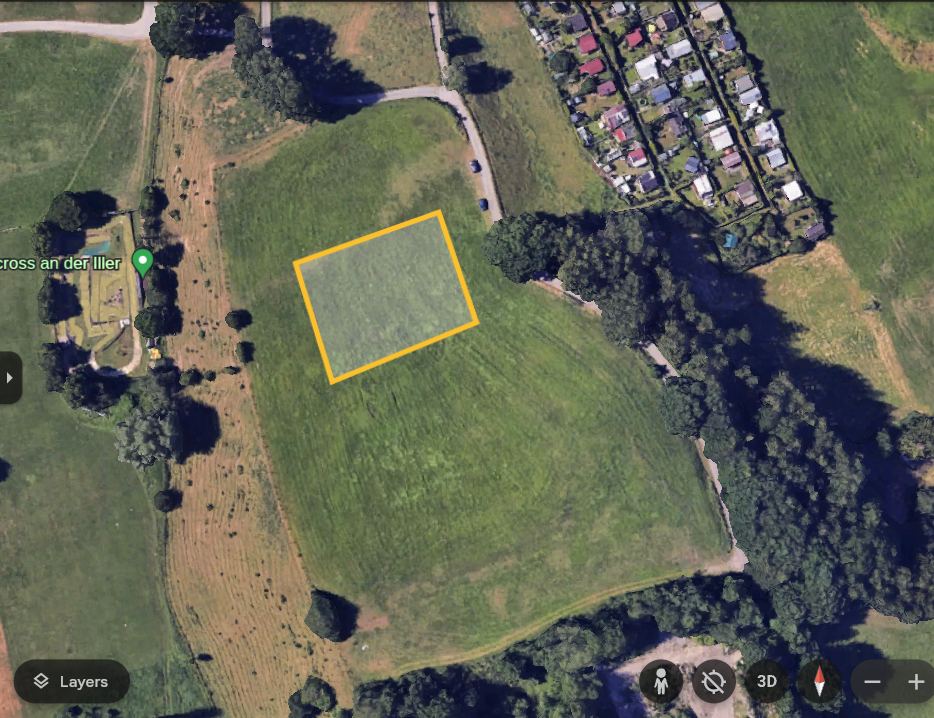
\includegraphics[width=\textwidth]{Images/real_robot/field_with_region.png}
            \caption{Selected Field Region}
        \end{subfigure} 
        &
        \begin{subfigure}{0.4\textwidth}
            \centering
            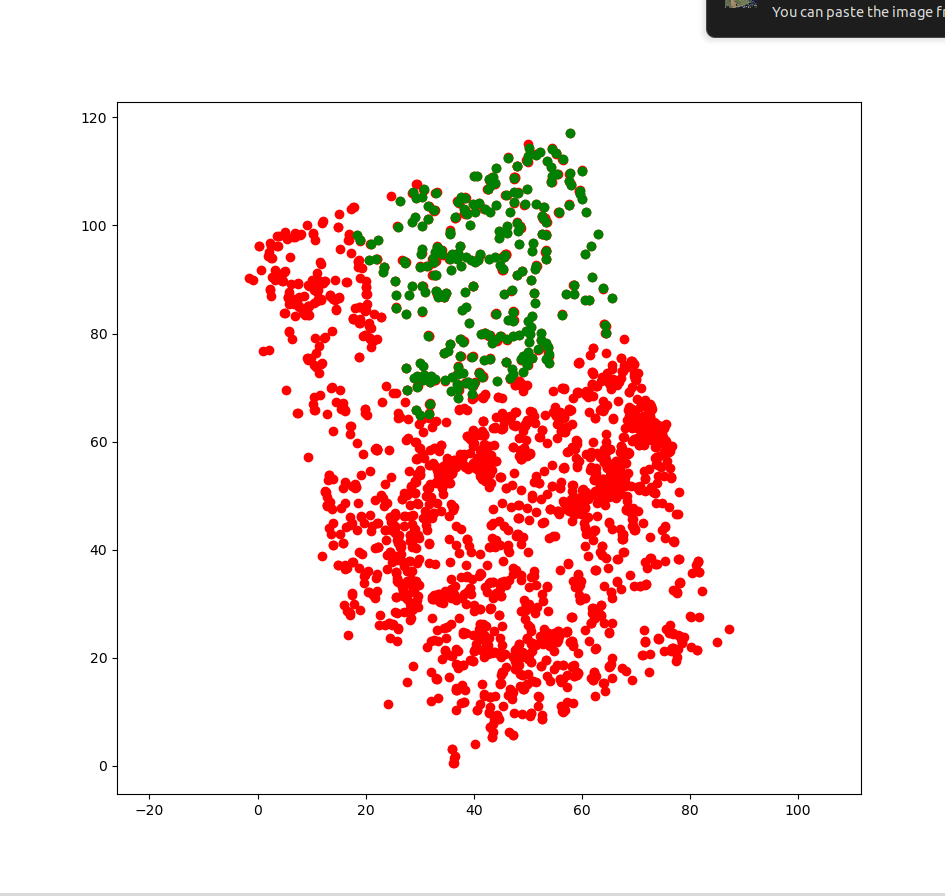
\includegraphics[width=\textwidth]{Images/real_robot/field_region_points.png}
            \caption{Points in the Region (Green)}
        \end{subfigure}
    \end{tabular}
    \caption{Selected field and points in the region.\label{fig:field_region}} 
\end{figure}


\vspace*{6mm}   


Apart from these adjustments, all the robot constraints and parameters were kept consistent with those discussed in the simulation setup. Two experimental cases were considered: one without obstacles and the other with obstacles. For the scenario involving obstacles, two polygonal obstacles (one concave and one convex) were introduced. The (\autoref{fig:two_obs_scenario}) depict both experimental scenarios. 


% selected field region.
\begin{figure}[H]
    \centering
    \begin{tabular}{cc} 
        \begin{subfigure}{0.4\textwidth}
            \centering
            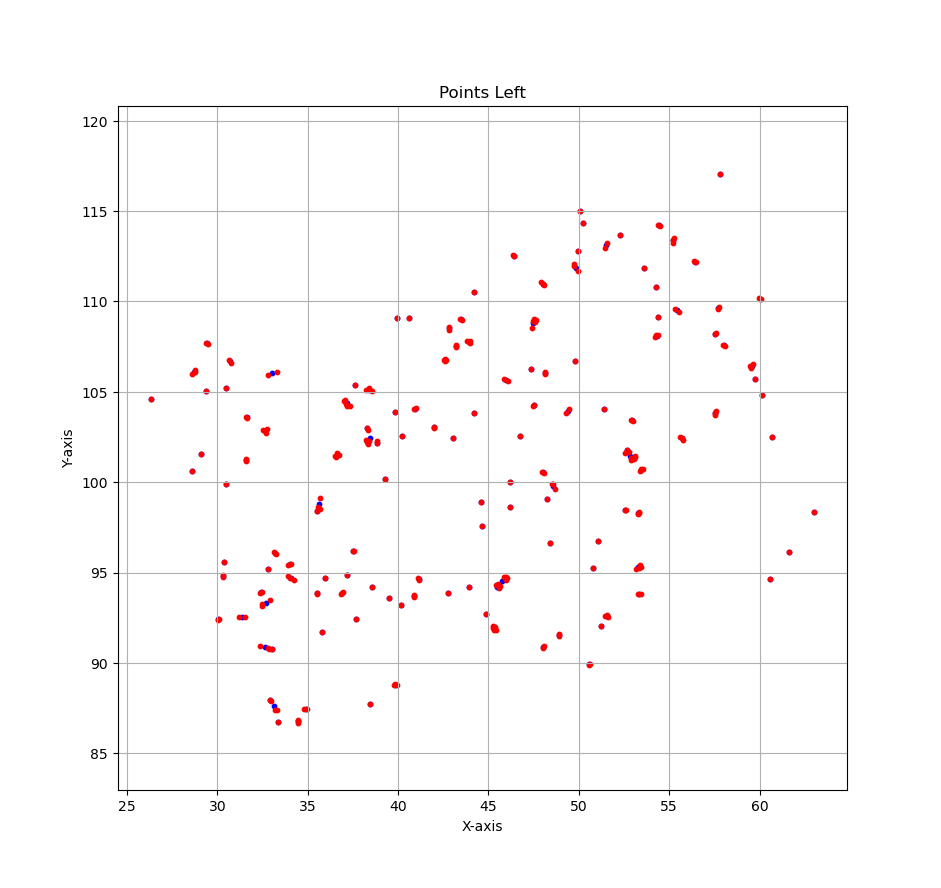
\includegraphics[width=\textwidth]{Images/real_robot/no_obs_scene.png}
            \caption{No obstacle scenario.}
        \end{subfigure} 
        &
        \begin{subfigure}{0.4\textwidth}
            \centering
            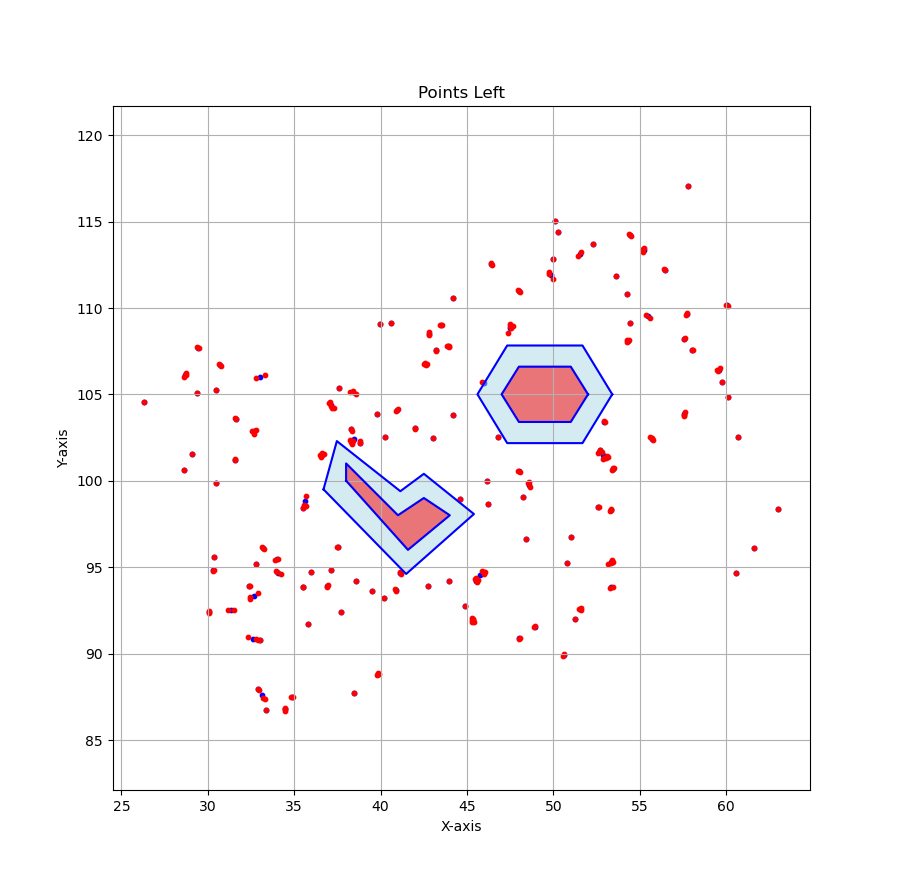
\includegraphics[width=\textwidth]{Images/real_robot/obs_scene.png}
            \caption{Two obstacles scenario.}
        \end{subfigure}
    \end{tabular}
    \caption{Distinct Environments.\label{fig:two_obs_scenario}} 
\end{figure}


\vspace*{6mm}   


The objective of demonstrating the CCP algorithm on a real robot platform is twofold: to showcase the alignment between the simulated global trajectory and the actual trajectory followed by the robot, and to evaluate the algorithm's effectiveness in weed removal. Specifically, the analysis focuses on how many weeds the robot successfully removes compared to the number planned by the global planner. Since the robot relies on its local planner, any deviation from the global planner's trajectory could result in missed weeds or the coverage of additional, unintended weed points.

\vspace*{6mm}   


This approach aims to highlight the practical applicability and robustness of the CCP algorithm in real-world agricultural settings, emphasizing its ability to adapt to various environmental conditions and obstacles while maintaining efficient operational performance.

\vspace*{6mm}   


\textbf{Real Robot Results and Analysis:}    

Initially, the real-world experiment was conducted on the first case without obstacles. Given that only 42\% coverage was used to demonstrate the results on the real robot, the global trajectory obtained from the simulation is depicted in (\autoref{fig:no_obs_traj}a). After executing the test on the real robot in the field, the actual path followed by the robot using the local planner is shown in (\autoref{fig:no_obs_traj}b).

% selected field region.
\begin{figure}[H]
    \centering
    \begin{tabular}{cc} 
        \begin{subfigure}{0.4\textwidth}
            \centering
            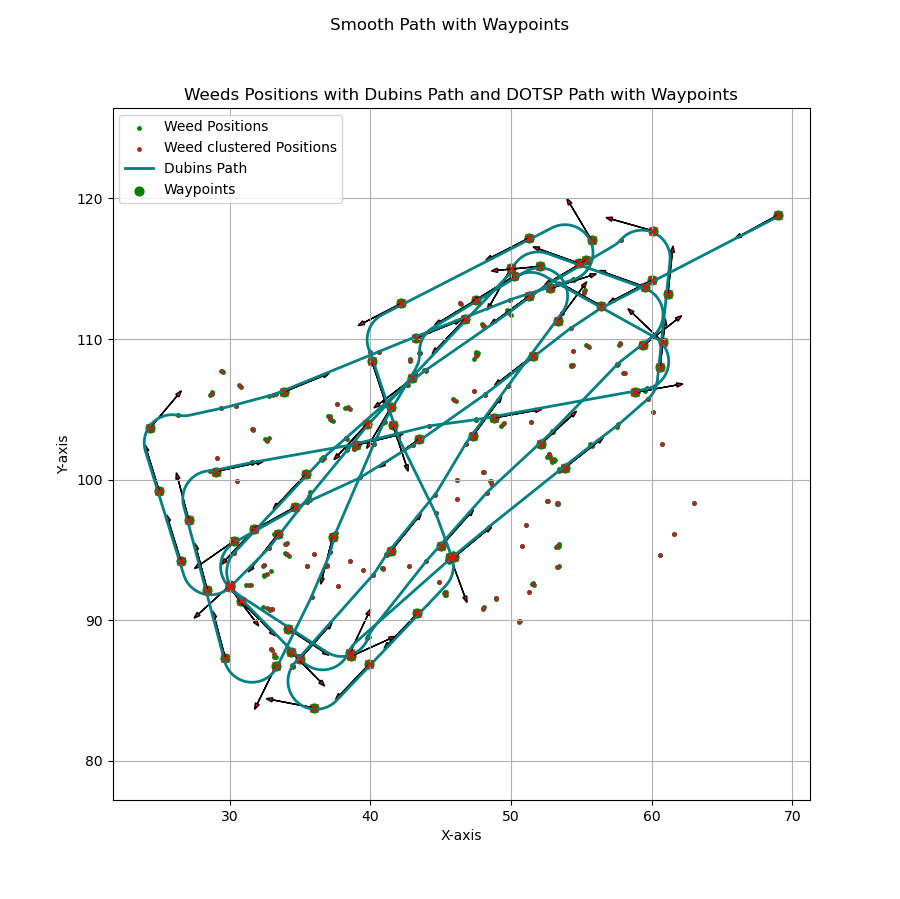
\includegraphics[width=\textwidth]{Images/real_robot/no_obs_path.png}
            \caption{Planned Path}
        \end{subfigure} 
        &
        \begin{subfigure}{0.4\textwidth}
            \centering
            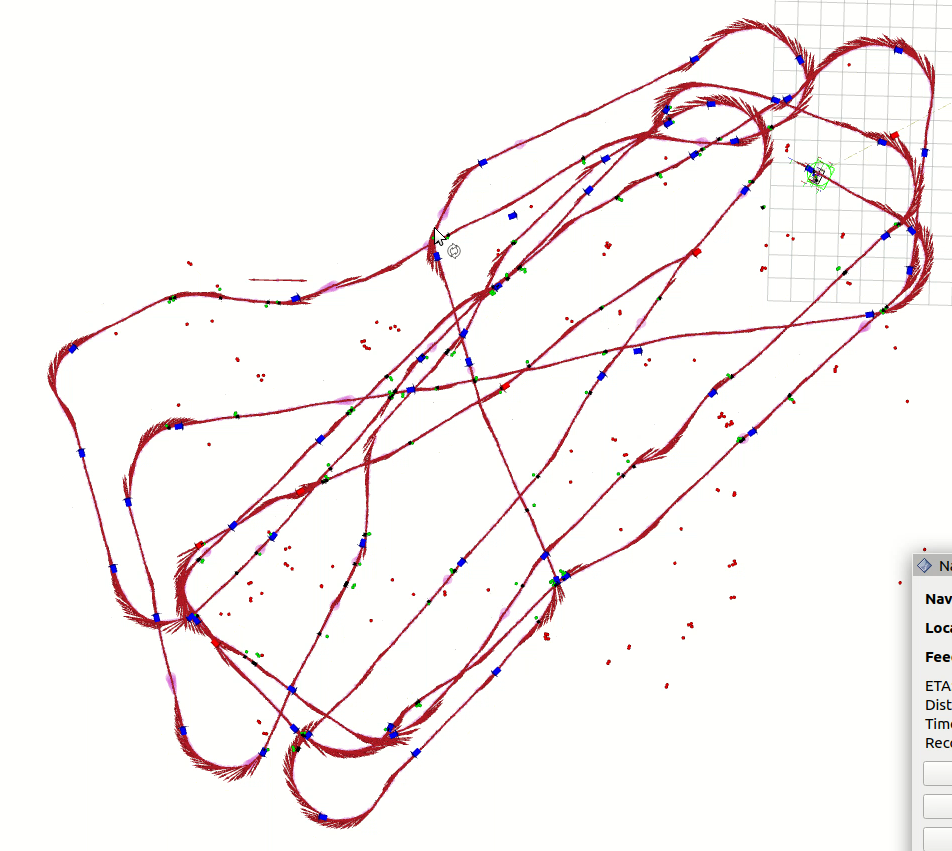
\includegraphics[width=\textwidth]{Images/real_robot/no_obs_real_path.png}
            \caption{Real Robot Path}
        \end{subfigure}
    \end{tabular}
    \caption{No obstacle Trajectories.\label{fig:no_obs_traj}} 
\end{figure}



\vspace*{6mm}   


The local planner initially identified 118 weeds for extraction, whereas the robot successfully removed 109 of these planned weeds. The discrepancy between the planned and actual removals arises from deviations in the local trajectories relative to the global trajectory. These deviations are primarily due to significant orientation differences between waypoints, which cause variations in the path of the local planner. Additionally, slight orientation adjustments made by the robot while navigating towards the waypoints and extracting weeds contribute to this difference. 

% The alignment between the global and local trajectories can be visualized in the figure below. To quantify this alignment, the absolute trajectory error (ATE) and relative pose error (RPE) were calculated, metrics commonly used in visual odometry literature. The ATE was x, and the RPE was y. Additional results, if available, can be visualized in the figure below.

% \textbf{Both trajectories on same  plot} 


\vspace*{6mm}   


Similarly, the same procedure was performed for the second case with obstacles. The global planned trajectory and the local trajectory from the real robot are illustrated in (\autoref{fig:obs_traj}). 

% selected field region.
\begin{figure}[H]
    \centering
    \begin{tabular}{cc} 
        \begin{subfigure}{0.4\textwidth}
            \centering
            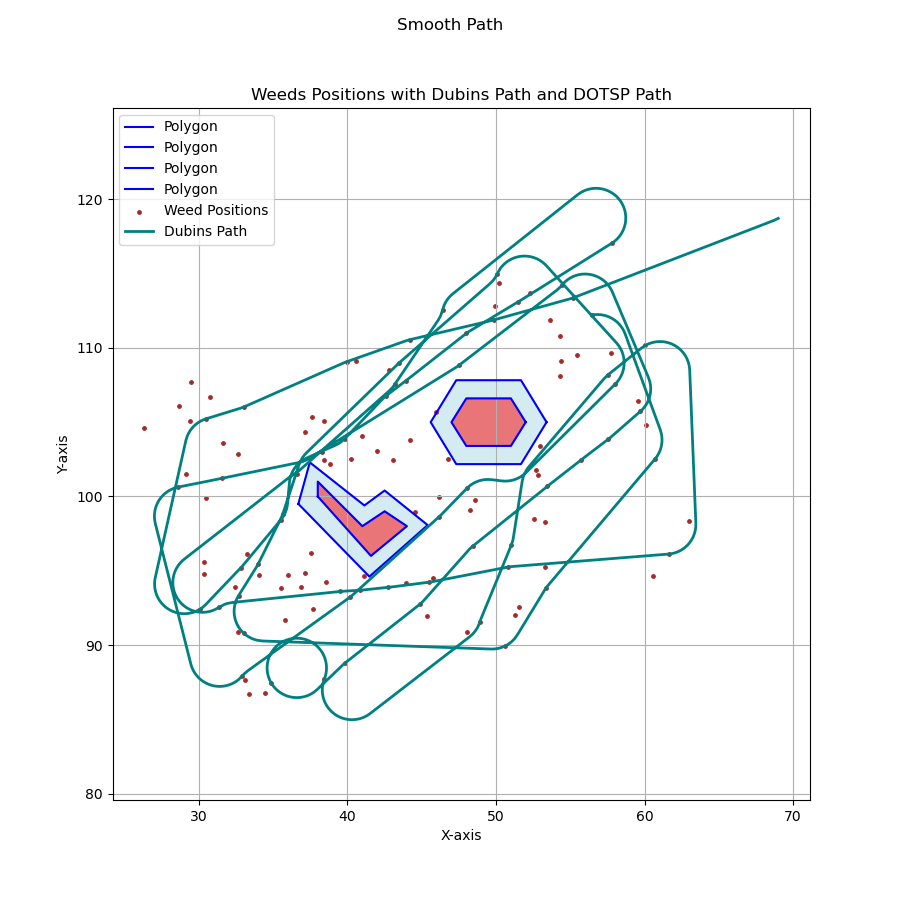
\includegraphics[width=\textwidth]{Images/real_robot/path_with_2_obs_v.png}
            \caption{Planned Path}
        \end{subfigure} 
        &
        \begin{subfigure}{0.4\textwidth}
            \centering
            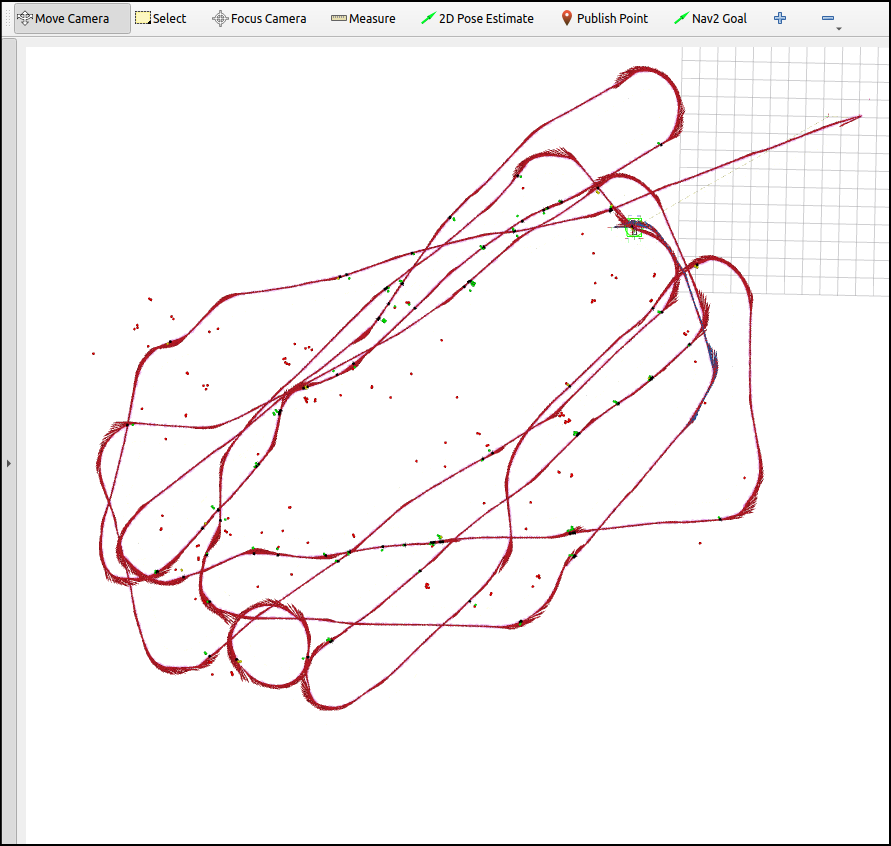
\includegraphics[width=\textwidth]{Images/real_robot/with_obs_real.png}
            \caption{Real Robot Path}
        \end{subfigure}
    \end{tabular}
    \caption{obstacle Trajectories.\label{fig:obs_traj}} 
\end{figure}

In this scenario, the local planner identified 101 weeds for extraction, whereas the robot successfully removed 84 of these weeds. The higher discrepancy in the number of weeds not covered in the presence of obstacles is attributed to the robot's need to navigate around these obstacles. This navigation often involves making curves, which leads to deviations between the planned path and the executed path, ultimately resulting in a lower success rate compared to scenarios without obstacles. However, despite this decrease, the success rate remains high, demonstrating the robustness of the algorithm, as it performs only slightly less efficiently than in obstacle-free scenarios.

\vspace*{6mm}   


The alignment between the two trajectories is illustrated in (\autoref{fig:traj_compare}). The absolute trajectory error was x, and the relative pose error was y. The success rate of weed removal is indirectly dependent on the trajectory error. Therefore, a lower error correlates with a higher success rate of weed removal. Typically, the success rate of weed removal is higher when the path is approximately straight, which aligns with the primary objective of maintaining a natural and approximately straight path.

Any additional results obtained are also visualized in the figure below.
\begin{figure}[htbp]
    \centering
    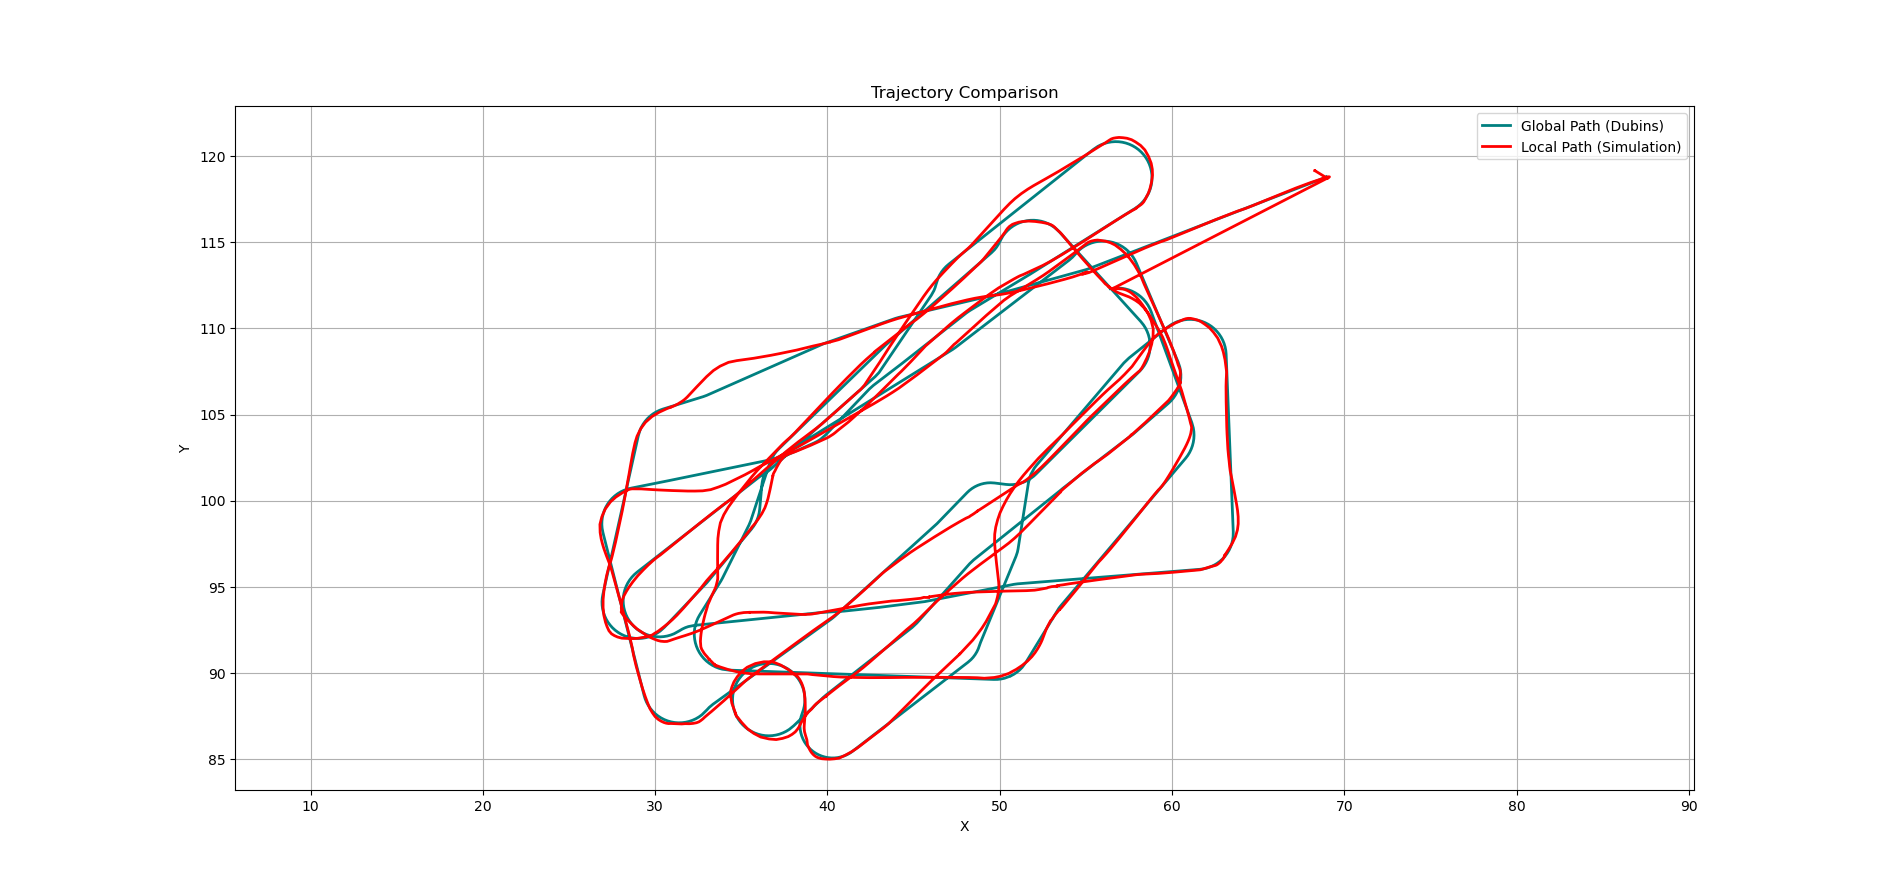
\includegraphics[width=\textwidth]{Images/real_robot/obs_compare.png}
    \caption{Trajector comparison.}
    \label{fig:traj_compare}
\end{figure}


Hence, it is evident from the above results that the robot is capable of closely following the global trajectory because the constraints are so well modelled in the global path to account the behavior of the local planner, thereby ensuring efficient and effective weed removal. The alignment between the global and local trajectories is crucial for achieving complete coverage, as any deviation could result in missed weeds or the coverage of unintended points. By minimizing this deviation, the proposed CCP algorithm can achieve optimal coverage, thus validating its practical applicability in real-world agricultural scenarios. The detailed analysis underscores the importance of trajectory alignment in achieving the desired operational outcomes.

\vspace*{6mm}   

To study the effect of non approximate straight paths on the planned and actually extracted weed points. The results from the graph search approach is also provided here. The scenario is the same as the one without obstacles we discussed earlier. The planned path obtained and the actual path followed by the robot are shown in the (\autoref{fig:gr_obs_traj}). The red dots represent the equidistant waypoints which robot follows to extract the weeds.

% selected field region.
\begin{figure}[H]
    \centering
    \begin{tabular}{cc} 
        \begin{subfigure}{0.4\textwidth}
            \centering
            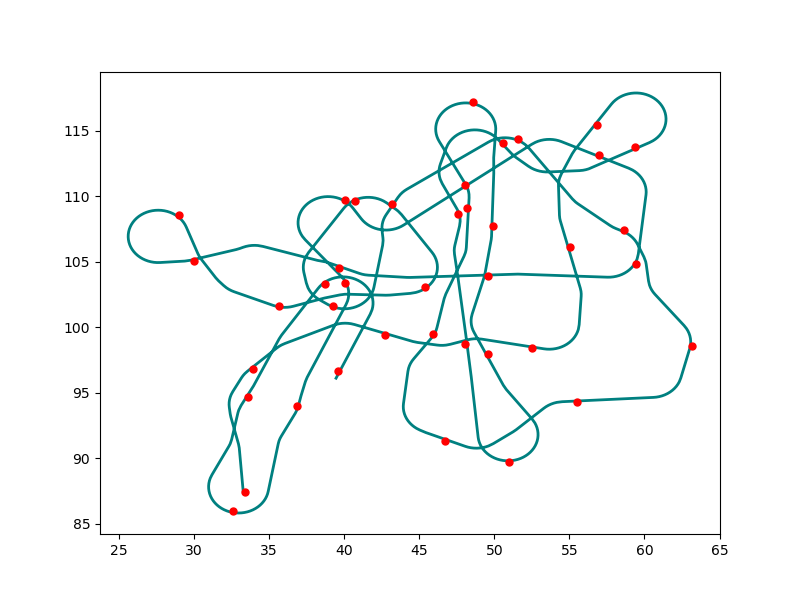
\includegraphics[width=\textwidth]{Images/real_robot/minh_planned.png}
            \caption{Planned Path}
        \end{subfigure} 
        &
        \begin{subfigure}{0.4\textwidth}
            \centering
            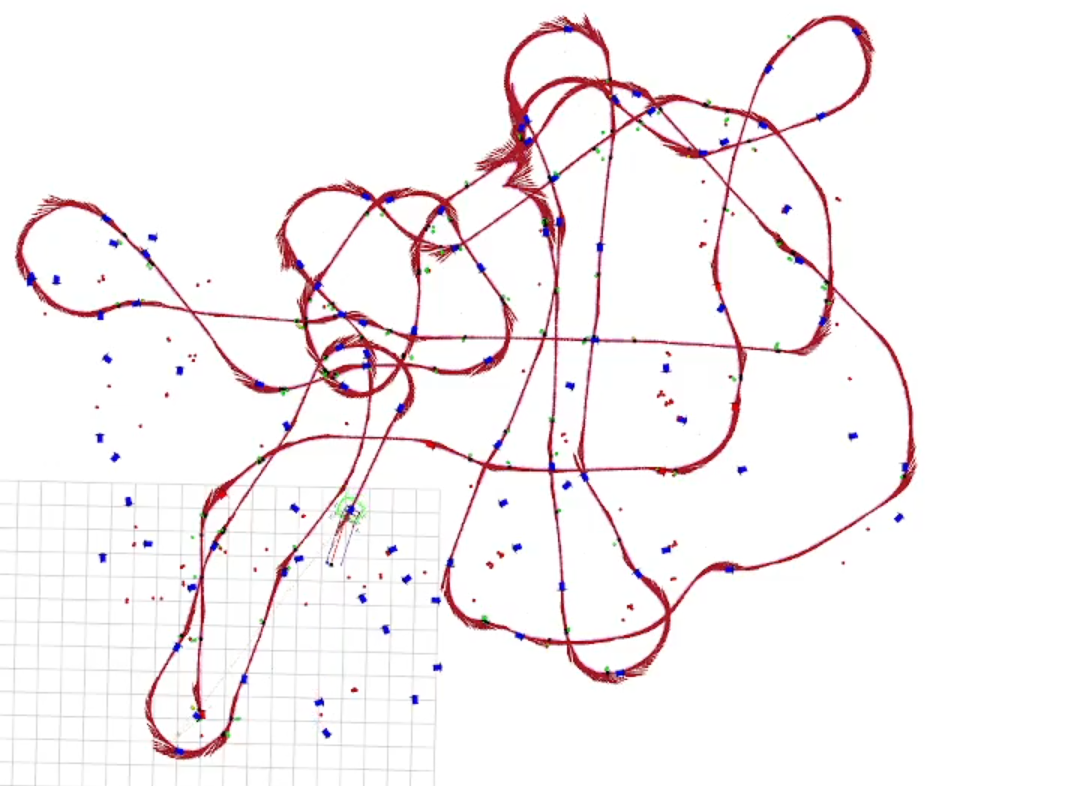
\includegraphics[width=\textwidth]{Images/real_robot/minh_simu.png}
            \caption{Real Robot Path}
        \end{subfigure}
    \end{tabular}
    \caption{Graph search no obstacle trajectories.\label{fig:gr_obs_traj}} 
\end{figure}


In this scenario, the number of weeds planned for extraction by the local planner was 191, while the number of weeds actually removed by the robot was 150. This discrepancy highlights the impact of non-approximately straight paths on the planned and actual weed extraction points. Curved paths result in greater orientation differences between waypoints, necessitating more adjustments by the robot while removing weeds and navigating these curves. Consequently, this leads to a larger deviation between the planned and actual weed extraction points, ultimately reducing the success rate of weed removal.

\vspace*{6mm}   

The graph search approach respects non-holonomic constraints but does not inherently prioritize approximately straight paths. One potential method to better align the trajectories in such cases is to provide more waypoints with shorter distances between them. However, this would require the robot to stop more frequently to adjust its orientation, select the next points for extraction by the local planner, and move to the next waypoint. While this could improve trajectory alignment, it would also increase field operation time and energy consumption.


The alignment between the two trajectories is illustrated in the (\autoref{fig:minh_traj_compare}). The absolute trajectory error was x, and the relative pose error was y. Any additional results obtained are also visualized in the figure below.

\begin{figure}[htbp]
    \centering
    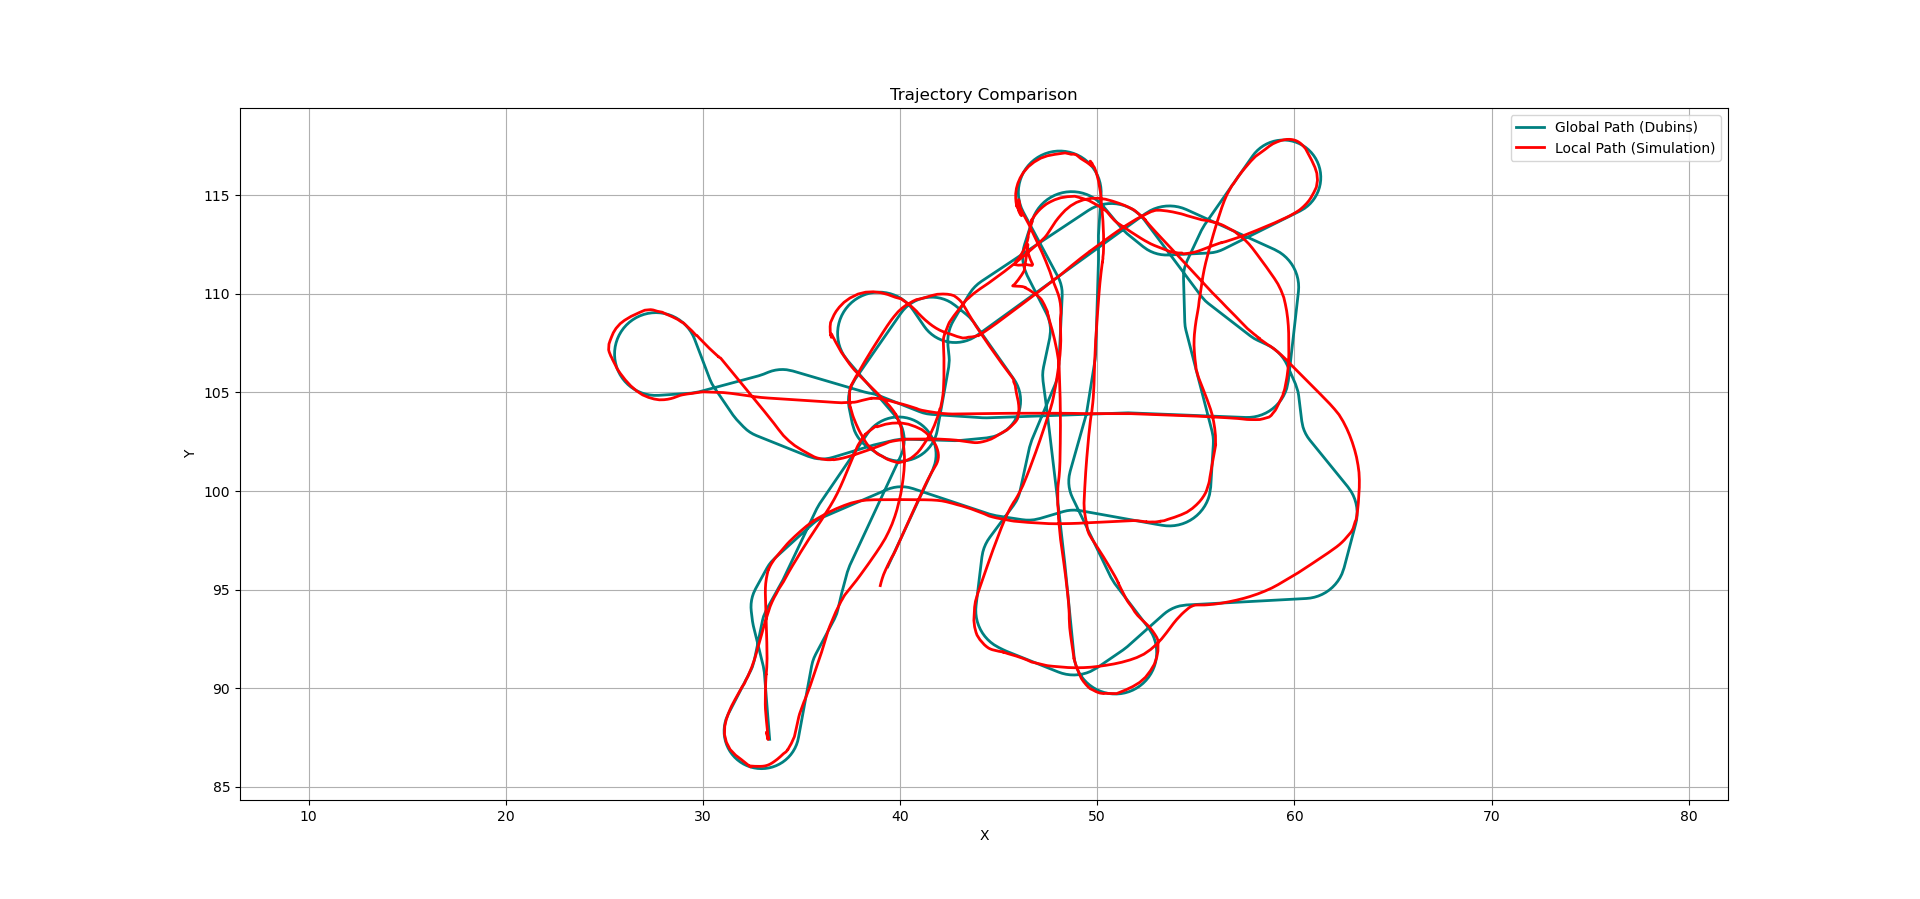
\includegraphics[width=\textwidth]{Images/real_robot/minhs_traj_2_better.png} 
    \caption{Trajector comparison.}
    \label{fig:minh_traj_compare}
\end{figure} 


\vspace*{6mm}    


\textbf{Analysis: } 

From the results, it can be summarized that the local planner (real robot) closely follows the global planner, demonstrating the accuracy of the global planner in modeling the robot's constraints in a manner that aligns well with the local planner. A key focus is the comparison between the number of weeds planned for extraction and the number of weeds actually removed. Ideally, these numbers should match as closely as possible, depending on the alignment between the local and global trajectories.

\vspace*{6mm}   

If the robot accurately follows the global trajectory, it will cover and extract all the planned weeds. Conversely, if there is a deviation, the robot may fail to extract some of the planned weeds and instead remove others that were not targeted. These additional weeds would have been covered in subsequent turns, and the missed weeds would remain uncovered, resulting in incomplete coverage.

\vspace*{6mm}   

Thus, the alignment between the global and local trajectories is crucial and can be assessed using the absolute trajectory error and relative pose error. These trajectory error metrics indirectly indicate the efficiency of the algorithm and the alignment between the global and local planners. Therefore, complete coverage is more likely if the trajectory deviation is minimal, whereas greater deviation compromises coverage completeness, leaving some weed points untreated.

\vspace*{6mm}   

By ensuring minimal deviation, the proposed CCP algorithm can achieve efficient and effective coverage, thus validating its applicability in real-world agricultural scenarios. The detailed analysis underscores the importance of trajectory alignment in achieving the desired operational outcomes.

\vspace*{6mm}   
